\chapter{Data Management}\label{chapter:data_management}


The data management needs can be differ by the use case. This can be done with different tools supplied by the rule engine. Therefore, developers benefit from different tools to realize their use cases by creating components. All the components needed is encapsulated within ontology of the use case. They all interact with each other to serve the needs of business logic. To keep ontology management simple, any components that owned by an ontology cannot be shared. However, they can be duplicated to other ontologies.

The data processing is done by the flows defined by the developer. The flows are chain of functioning blocks which are called nodes. These flows can be easily implemented by using query engine API directly or the user interface. 

The classification of data is done in completely independent application which is called Ontology Engine. Ontology Engine is loosely coupled with the rest of the system. It classify data by using Web Ontology Language(OWL) and HermiT OWL Reasoner. In entire system, when to classify data and what to do with the classified data is defined in flows. Flows communicate with Ontology Engine whenever it is need by using correct MQTT topics.

Currently, there are three way to handle with resulted data. They can be stored in ElasticSearch database, published in defined topics of any MQTT broker or stored in the nodes of the flows for further calculation.

\section{Ontology Management}

As described before, an ontology can have different components to manage different needs. In figure \ref{fig:ontology_components}, the components belong to an ontology is shown. An ontology can have as many flow it is needed to manage data process. Each flow is consist of various nodes. These nodes can send or receive data to each other inside of the flow. However, they cannot be connected with the nodes in different flows. Therefore, encapsulation of the data traversing inside a flow is sustained. Ontologies also own a OWL document with information to be used in the classification of data. This document stored and managed by Ontology Engine while all the flows are managed in Ontology Manager. Therefore, the inter-communication between two different subsystem shall be succeeded. 


\begin{figure}[H]
  \centering
  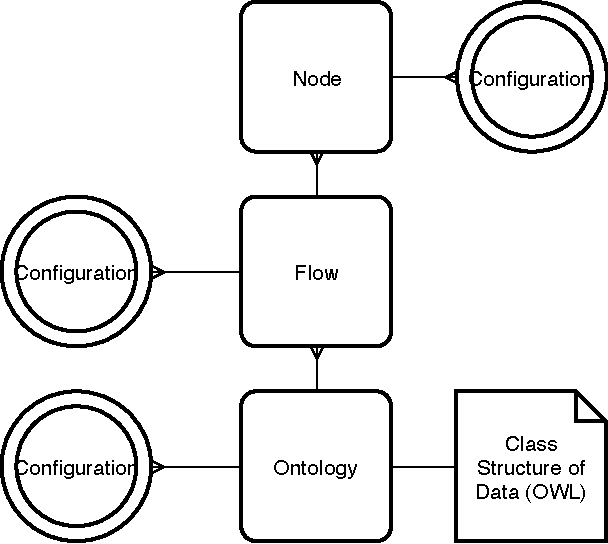
\includegraphics[width=0.7\textwidth,height=\textheight,keepaspectratio]{figures/components_of_ontology.pdf}
  \caption[Ontology Components]{Components of an Ontology}\label{fig:ontology_components}
\end{figure}

All these subsystems can be located in different machines in cloud without any common resource. Nevertheless, they have to be aware of where each subsystem is located and how they can communicate with them. Most of the communication between components are done in a structured way. The flows send data to classify to Ontology Engine by using "/ontology/query/<Ontology ID>" MQTT topic. Then, Ontology Manager returns the received data back to flows by using "/ontology/classified/<Ontology ID>/<Class Name>" MQTT topic. If a received data belong to more than one class, the same data is published to topics of all matched classes.

In figure \ref{fig:ontology_creation}, the sequence diagram for a user tries to create a new ontology using web application interface is shown. The web application serves for usability purposes with a simple user interface. It is also possible for a user to surpass the web application and use query manager directly within their needs. Initial communication configuration of components is set by Query Manager in their initialization process. It balances and pairs each ontology to existing Ontology Engines and Ontology Managers.  Besides to initial configuration, reallocation of a component to different machine or fault in an existing system might cause reconfiguration of the components. For this purpose, Query Manager also notifies and reconfigures each component to how to communicate with their fellow component when needed. 

\begin{figure}[H]
  \centering
  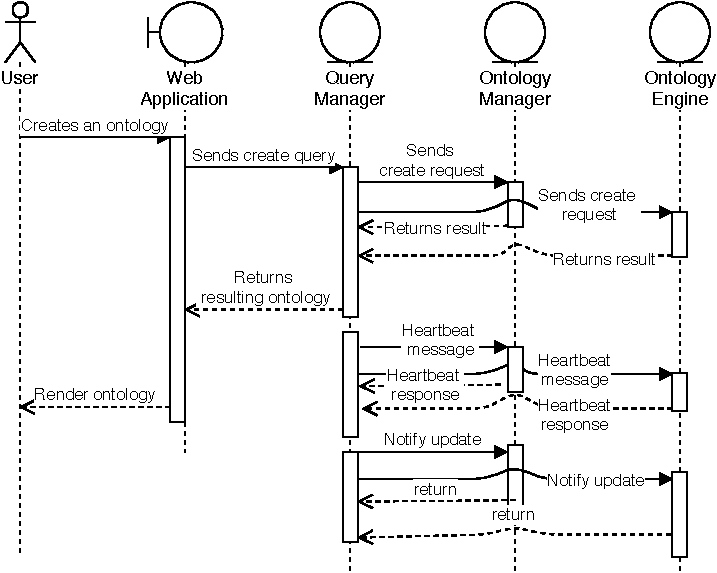
\includegraphics[width=\textwidth,height=\textheight,keepaspectratio]{figures/ontology_creation.pdf}
  \caption[Sequence Diagram for Ontology Creation]{Creation Diagram of an Ontology}\label{fig:ontology_creation}
\end{figure}



\subsection{Data Classification in Ontologies}

Knowledge base of how to classify a received data is kept in Ontology Engine. This knowledge base is defined in a extendable way with OWL. Moreover, each ontology has its own knowledge base to work with. Therefore, any user can extend their classification logic by extending related OWL file. Thanks to these extensions, more complex and specific classification can be made to achieve the goals of business logic.

The most important OWL class which is defined and used in Ontology Engine is "IoTOntology:Data". For each received data, a new individual of IoTOntology:Data class of related ontology is created. For each field existing in data, class named as "IoTOntology:<Field Name>Field", a new indiviudal of that class and a data property named as "IoTOntology:has<Field Name>Value" are created if they do not exist in current ontology model. Then, a object property assertion is added to newly generated data individual with "IoTOntology:hasField" object property and field individual. A data property assertion  is also added by using related data and the value itself.


\lstinputlisting[language=json,caption=Sample Received Data,label={lst:sample_data}]{code_snippets/sample_data_query.json}

JSON object given in listing \ref{lst:sample_data} can be taken as an example. Ontology engine will create a new data individual in ontology for this data. In figure \ref{fig:data_ontology}, generated individual with its properties from this data is shown. This generated individual is used by the reasoner to classify data.
\begin{figure}[H]
  \centering
  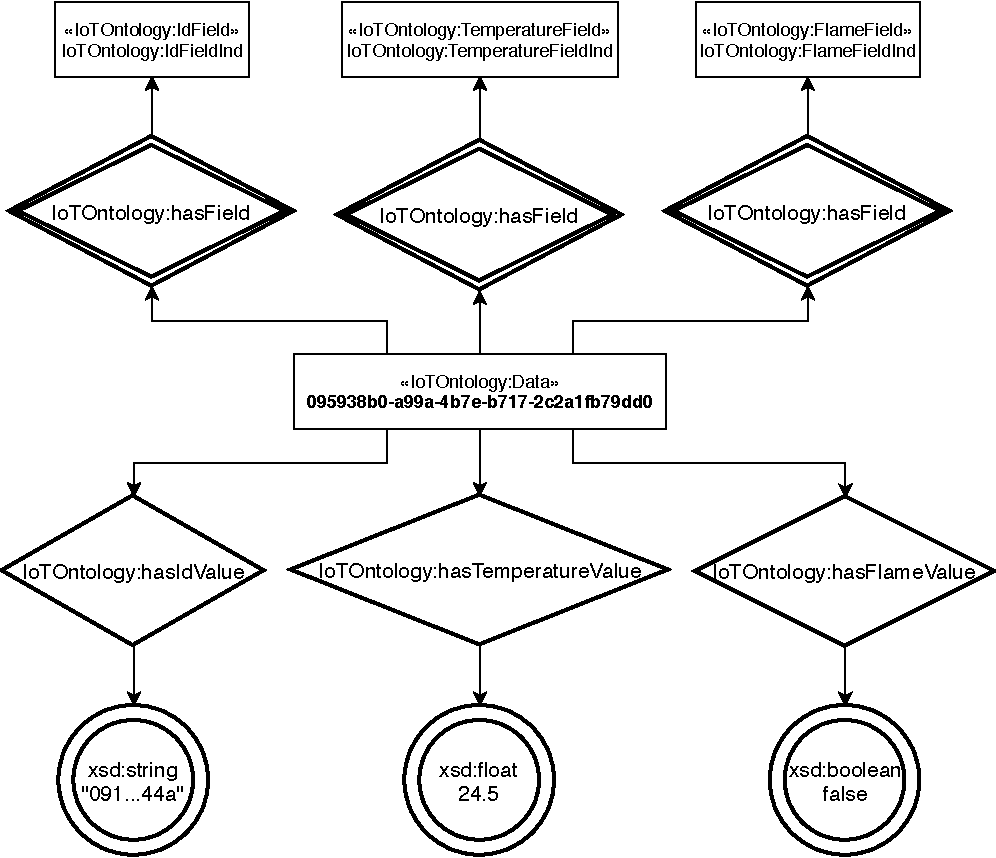
\includegraphics[width=\textwidth,height=\textheight,keepaspectratio]{figures/sample_data_ontology.pdf}
  \caption[Sample Ontology Representation of Data]{Generated Individual of Received Data}\label{fig:data_ontology}
\end{figure}

With help of HermiT reasoner, classes that a data belongs to is inferred. To make integration with Hardware Abstraction Layer, data types that are generated by the sensors are predefined in each OWL file. By just using this as our knowledge base without any modification, Ontology Engine can deduct that the data is belong to all FlameData, TemperatureData, DataWithTemperatureField and DataWithFlameField classes. In OWL snippet in listing \ref{lst:data_hierarchy}; OWL classes, properties and restrictions related to this reasoning process can be found.

\lstinputlisting[language=XML,caption=Flame and Temperature Data Classes from OWL File,label={lst:data_hierarchy}]{code_snippets/sample_data_ontology.owl}

In figure \ref{proof:data_proof}, the deduction process for the reasoning of the received data can be found. By the definition of IoTOntology:DataWithFlameField and IoTOntology: DataWithTemperatureField classes, every IoTOntology:Data individual which has at least one temperature or flame field is belong to IoTOntology:DataWithFlameField or IoTOntology:DataWithTemperatureField classes. Therefore,  IoTOntology:Data individual is also an individual of both IoTOntology:DataWithFlameField and IoTOntology:DataWithTemperatureField classes. Moreover, it also belongs IoTOntology:FlameData and IoTOntology:Temperature classes since they are super-classes of IoTOntology: DataWithFlameField and IoTOntology:DataWithTemperatureField classes. Hiearchy of IoTOntology:FlameData and IoTOntology:Temperature classes can be seen in figure  \ref{fig:data_hierarchy}.
\begin{figure}[H]
$id = $"095938b0-a99a-4b7e-b717-2c2a1fb79dd0"\newline
$D = Data$\newline
$TDf = DataWithTemperatureField$\newline
$TD = TemperatureData$\newline
$T = TemperatureField$ \newline
$T* = TemperatureField(TemperatureFieldInd)$\newline
$FDf = DataWithFlameField$\newline
$FD = FlameData$\newline
$F = FlameField$\newline
$F* = FlameField(FlameFieldInd)$\newline
\begin{prooftree}
    \AxiomC{$TDf(x) \to TD(x)$}
    \AxiomC{$hasField(D(id), T*)$}
    \AxiomC{$hasField(D(x), T) \equiv  TDf(x)$}
    \BinaryInfC{$TDf(id)$}
    \BinaryInfC{$TD(id)$}
\end{prooftree}
\begin{prooftree}
    \AxiomC{$FDf(x) \to FD(x)$}
    \AxiomC{$hasField(D(id), F*)$}
    \AxiomC{$hasField(D(x), F) \equiv  FDf(x)$}
    \BinaryInfC{$FDf(id)$}
    \BinaryInfC{$FD(id)$}
\end{prooftree}
  \caption[Reasoning of a Sample Data]{Reasoning of Received Data}\label{proof:data_proof}
\end{figure}
\begin{figure}[H]
  \centering
  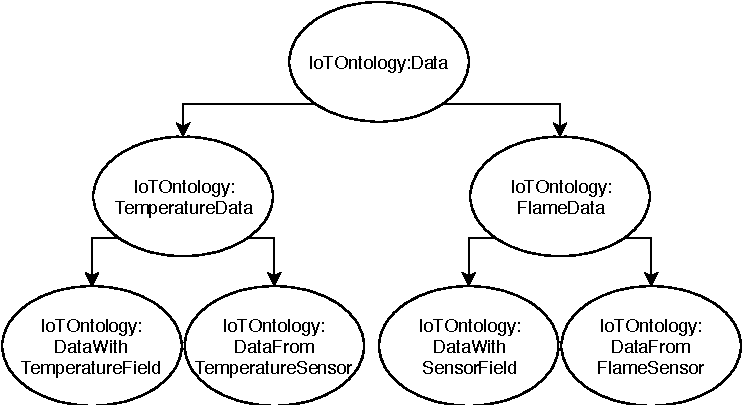
\includegraphics[width=\textwidth,height=\textheight,keepaspectratio]{figures/data_hierarchy.pdf}
  \caption[Data Class Hierarchy]{Hierarchy of Flame and Temperature Data Classes}\label{fig:data_hierarchy}
\end{figure}


\section{Process of Data in Ontologies}\label{section:data_process}

Ontology manager manages every steps in data process. The data processing in ontologies are handled by the flows and their nodes. The flows manages and encapsulates their nodes. There are three types of nodes with their own subtypes. These types are sink nodes, middle nodes and source nodes. Data is gathered, processed and sinked by these nodes of flows. The source nodes are responsible for listening for coming data. They redirect data that they have gathered to their proceeding nodes. The middle nodes handles all the required proccess on the data to generate resulting data. They execute their proceeding nodes with their resulting data. The proceeding nodes cannot have information about what is the data like in previous steps. They can only reach data generated by their prior nodes. In sink nodes, the resulted data is sinked from flow and Ontology Manager to any other system.

\begin{figure}[H]
  \centering
  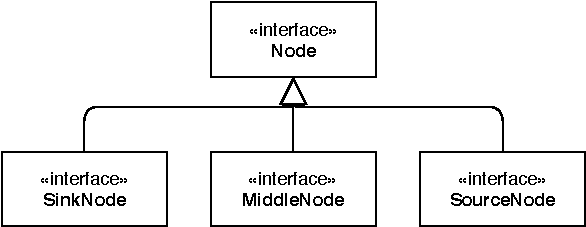
\includegraphics[width=\textwidth,height=\textheight,keepaspectratio]{figures/node_types.pdf}
  \caption[Node Types]{Three Node Type}\label{fig:node_types}
\end{figure}

An ontology can have more than flow with each doing their own processes on data. The flows cannot share a node or cannot pass data to each other directly. Nevertheless, its possible to pass data by making a source node to listen a message coming over MQTT topic and sinking the data from a sink node of another from to the same MQTT topic.

The flows also manage caching functionality and self-adapt accordingly the data reached to their source nodes and resulted data in sink nodes. When a data reached to any source node of a flow, the flow checks whether this data is cached previously. If it is cached in the cache of he flow, the sink nodes are executed with cached data directly bypassing middle nodes. 

\subsection{Nodes for Data Processes}

As mentioned in the section \ref{section:data_process}, there are three main types of nodes. These are sink, middle and source nodes. Moreover, each of these types has their own sub-types.
\begin{figure}[H]
  \centering
  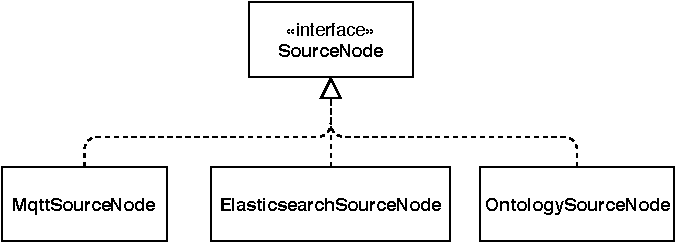
\includegraphics[width=\textwidth,height=\textheight,keepaspectratio]{figures/source_nodes.pdf}
  \caption[Source Node Types]{Source Node Types}\label{fig:source_nodes}
\end{figure}
\begin{figure}[H]
  \centering
  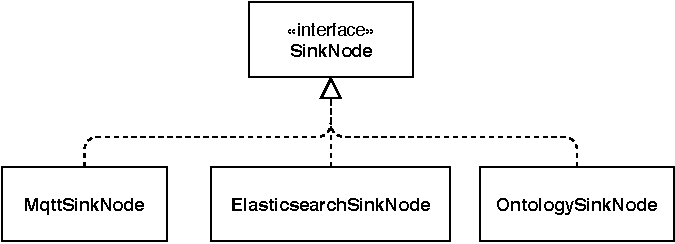
\includegraphics[width=\textwidth,height=\textheight,keepaspectratio]{figures/sink_nodes.pdf}
  \caption[Sink Node Types]{Sink Node Types}\label{fig:sink_nodes}
\end{figure}

\subsection{Self-Adaptation of Flows}

\subsection{Performance Issues and Solutions of Rules}

